\documentclass{beamer}

\author[D. Abercrombie]{
  Daniel Abercrombie, \\
  Guillelmo G\'omez-Ceballos, \\
  Dymtro Kovalskyi, \\
  Benedikt Maier, \\
  Christoph Paus
}

\title{\bf \sffamily B-Jet Regression and Di-jet Response}
\date{\today}

\usecolortheme{dove}

\usepackage[absolute,overlay]{textpos}
\usefonttheme{serif}
\usepackage{appendixnumberbeamer}
\usepackage{isotope}
\usepackage{hyperref}
\usepackage[english]{babel}
\usepackage{amsmath}
\setbeamerfont{frametitle}{size=\Large,series=\bf\sffamily}
\setbeamertemplate{frametitle}[default][center]
\usepackage{siunitx}
\usepackage{tabularx}
\usepackage{makecell}
\usepackage{comment}

\setbeamertemplate{navigation symbols}{}
\usepackage{graphicx}
\usepackage{color}
\setbeamertemplate{footline}[text line]{\parbox{1.083\linewidth}{\footnotesize \hfill \insertshortauthor \hfill \insertpagenumber /\inserttotalframenumber}}
\setbeamertemplate{headline}[text line]{\parbox{1.083\linewidth}{\footnotesize \hspace{-0.083\linewidth} \textcolor{blue}{\sffamily \insertsection \hfill \insertsubsection}}}

\IfFileExists{/Users/dabercro/GradSchool/Presentations/MIT-logo.pdf}
             {\logo{\includegraphics[height=0.5cm]{/Users/dabercro/GradSchool/Presentations/MIT-logo.pdf}}}
             {\logo{\includegraphics[height=0.5cm]{/home/dabercro/MIT-logo.pdf}}}

\usepackage{changepage}

\newcommand{\beginbackup}{
  \newcounter{framenumbervorappendix}
  \setcounter{framenumbervorappendix}{\value{framenumber}}
}
\newcommand{\backupend}{
  \addtocounter{framenumbervorappendix}{-\value{framenumber}}
  \addtocounter{framenumber}{\value{framenumbervorappendix}}
}

\graphicspath{{figs/}}

\newcommand{\link}[2]{\href{#2}{\textcolor{blue}{\underline{#1}}}}
\newcommand{\clink}[2]{\link{#1}{http://t3serv001.mit.edu/~dabercro/redir/?k=#2}}}

\newcommand{\twofigs}[4]{
  \begin{columns}
    \begin{column}{0.5\linewidth}
      \centering
      \textcolor{blue}{#1} \\
      \includegraphics[width=\linewidth]{#2}
    \end{column}
    \begin{column}{0.5\linewidth}
      \centering
      \textcolor{blue}{#3} \\
      \includegraphics[width=\linewidth]{#4}
    \end{column}
  \end{columns}
}

\newcommand{\fourfigs}[8]{
  \begin{columns}
    \begin{column}{0.3\linewidth}
      \centering
      \textcolor{blue}{#1} \\
      \includegraphics[width=\linewidth]{#2} \\
      \textcolor{blue}{#3} \\
      \includegraphics[width=\linewidth]{#4}
    \end{column}
    \begin{column}{0.3\linewidth}
      \centering
      \textcolor{blue}{#5} \\
      \includegraphics[width=\linewidth]{#6} \\
      \textcolor{blue}{#7} \\
      \includegraphics[width=\linewidth]{#8}
    \end{column}
  \end{columns}
}

\newcommand{\ttbar}{\ensuremath{t\bar{t}}}
\newcommand{\bbbar}{\ensuremath{b\bar{b}}}

\begin{document}

\begin{frame}
  \titlepage
\end{frame}

\begin{frame}
  \frametitle{Introduction}

  \begin{itemize}
  \item Extensions for DY samples in NanoAODv7 are available now,
    so I ran one more pass of the smearing fits
  \item 2016 now does suggest some smearing, though it's much smaller than the other samples
  \end{itemize}

  More comfortable using Xbb framework

  \begin{itemize}
  \item Plots for $Z\rightarrow \ell\ell$ response are finished
  \item I wasn't saving quite enough information to get the top mass using unregressed b-jets
    \begin{itemize}
    \item Might not be ready for Wednesday, but doesn't seem like a show stopper
    \end{itemize}
  \item Signal mass histograms are made,
    fit should be ready today
  \end{itemize}

\end{frame}

\begin{frame}
  \frametitle{The Usual Smearing Plots}

  \vfill
  \centering
  Before Smearing
  \vfill

  \begin{columns}
    \begin{column}{0.33\linewidth}
      \centering
      \textcolor{blue}{2016}
      \includegraphics[width=\linewidth]{figs/200619_smear_200619_2016_divmean/resolution_jet1_adjusted_response_smear_0.pdf}
    \end{column}
    \begin{column}{0.34\linewidth}
      \centering
      \textcolor{blue}{2017}
      \includegraphics[width=\linewidth]{figs/200619_smear_200619_2017_divmean/resolution_jet1_adjusted_response_smear_0.pdf}
    \end{column}
    \begin{column}{0.33\linewidth}
      \centering
      \textcolor{blue}{2018}
      \includegraphics[width=\linewidth]{figs/200619_smear_200619_2018_divmean/resolution_jet1_adjusted_response_smear_0.pdf}
    \end{column}
  \end{columns}

\end{frame}

\begin{frame}
  \frametitle{The Usual Smearing Plots}

  \vfill
  \centering
  Nominal Smearing
  \vfill

  \begin{columns}
    \begin{column}{0.33\linewidth}
      \centering
      \textcolor{blue}{2016}
      \includegraphics[width=\linewidth]{figs/200619_smear_200619_2016_divmean/resolution_jet1_adjusted_response_smeared_scaled_nominal_smear_0.pdf}
    \end{column}
    \begin{column}{0.34\linewidth}
      \centering
      \textcolor{blue}{2017}
      \includegraphics[width=\linewidth]{figs/200619_smear_200619_2017_divmean/resolution_jet1_adjusted_response_smeared_scaled_nominal_smear_0.pdf}
    \end{column}
    \begin{column}{0.33\linewidth}
      \centering
      \textcolor{blue}{2018}
      \includegraphics[width=\linewidth]{figs/200619_smear_200619_2018_divmean/resolution_jet1_adjusted_response_smeared_scaled_nominal_smear_0.pdf}
    \end{column}
  \end{columns}

\end{frame}

\begin{frame}
  \frametitle{The Usual Smearing Plots}

  \vfill
  \centering
  Additional Smearing
  \vfill

  \begin{columns}
    \begin{column}{0.33\linewidth}
      \centering
      \textcolor{blue}{2016}
      \includegraphics[width=\linewidth]{figs/200619_smear_200619_2016_divmean/resolution_jet1_adjusted_response_smeared_scaled_up_smear_0.pdf}
    \end{column}
    \begin{column}{0.34\linewidth}
      \centering
      \textcolor{blue}{2017}
      \includegraphics[width=\linewidth]{figs/200619_smear_200619_2017_divmean/resolution_jet1_adjusted_response_smeared_scaled_up_smear_0.pdf}
    \end{column}
    \begin{column}{0.33\linewidth}
      \centering
      \textcolor{blue}{2018}
      \includegraphics[width=\linewidth]{figs/200619_smear_200619_2018_divmean/resolution_jet1_adjusted_response_smeared_scaled_up_smear_0.pdf}
    \end{column}
  \end{columns}

\end{frame}

\begin{frame}
  \frametitle{Numbers}

  The smearing applicator has been updated: \url{https://github.com/dabercro/hbb/blob/master/nanoslimmer/applysmearing/applysmearing.py}

  \vfill
  \begin{center}
    \begin{tabular}{|l|c|c|}
      \hline
      Year & MC Scaling & Smearing \\
      \hline
      2016 & $1.013 \pm 0.014$ & $2.9 \pm 4.7 \%$ \\
      2017 & $1.017 \pm 0.021$ & $5.8 \pm 6.6 \%$ \\
      2018 & $0.985 \pm 0.019$ & $8.0 \pm 7.3 \%$ \\
      \hline
    \end{tabular}
  \end{center}

  \vfill
  List of things I would check for 2016:
  \begin{itemize}
  \item Tune is different for 2016, do the normal jets require less smearing?
  \item Are the variables that go into the DNN correlated more correctly in 2016?
  \end{itemize}

\end{frame}

\begin{frame}
  \frametitle{$p_T$ Balance}

  \begin{columns}
    \begin{column}{0.33\linewidth}
      \centering
      \textcolor{blue}{No Regression}
      \includegraphics[width=\linewidth]{figs/200622_Zll2018_runplot-v5/Zhf_medhigh_Zll__ptBalance_noReg_.pdf}
    \end{column}
    \begin{column}{0.34\linewidth}
      \centering
      \textcolor{blue}{With Regression}
      \includegraphics[width=\linewidth]{figs/200622_Zll2018_runplot-v5/Zhf_medhigh_Zll__ptBalance_.pdf}
    \end{column}
    \begin{column}{0.33\linewidth}
      \centering
      \textcolor{blue}{With Kinematic Fit}
      \includegraphics[width=\linewidth]{figs/200622_Zll2018_runplot-v5/Zhf_medhigh_Zll__ptBalance_kinfit_.pdf}
    \end{column}
  \end{columns}

\end{frame}

\begin{frame}
  \frametitle{Di-jet Mass Histograms}

  \begin{columns}
    \begin{column}{0.33\linewidth}
      \centering
      \textcolor{blue}{No Regression}
      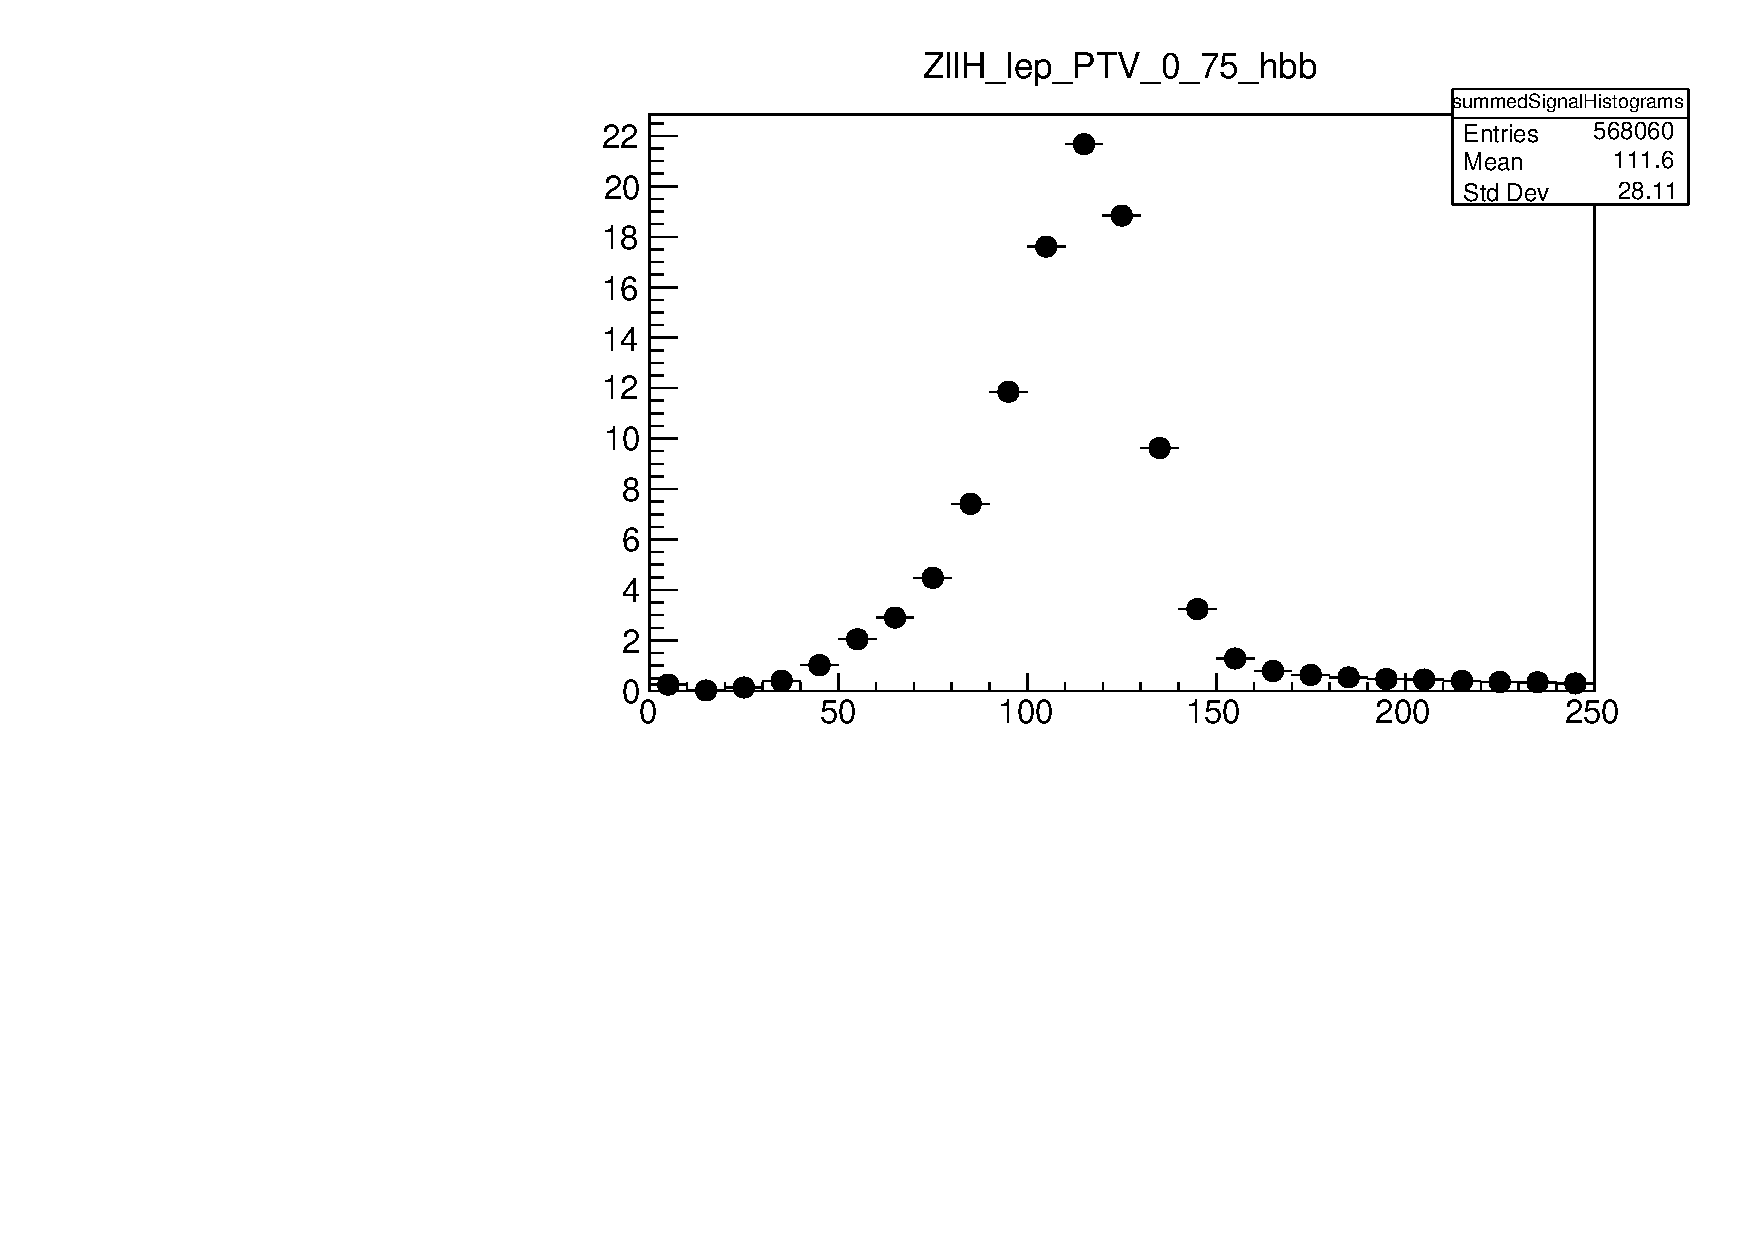
\includegraphics[width=\linewidth]{figs/noreg.pdf}
    \end{column}
    \begin{column}{0.34\linewidth}
      \centering
      \textcolor{blue}{With Regression}
      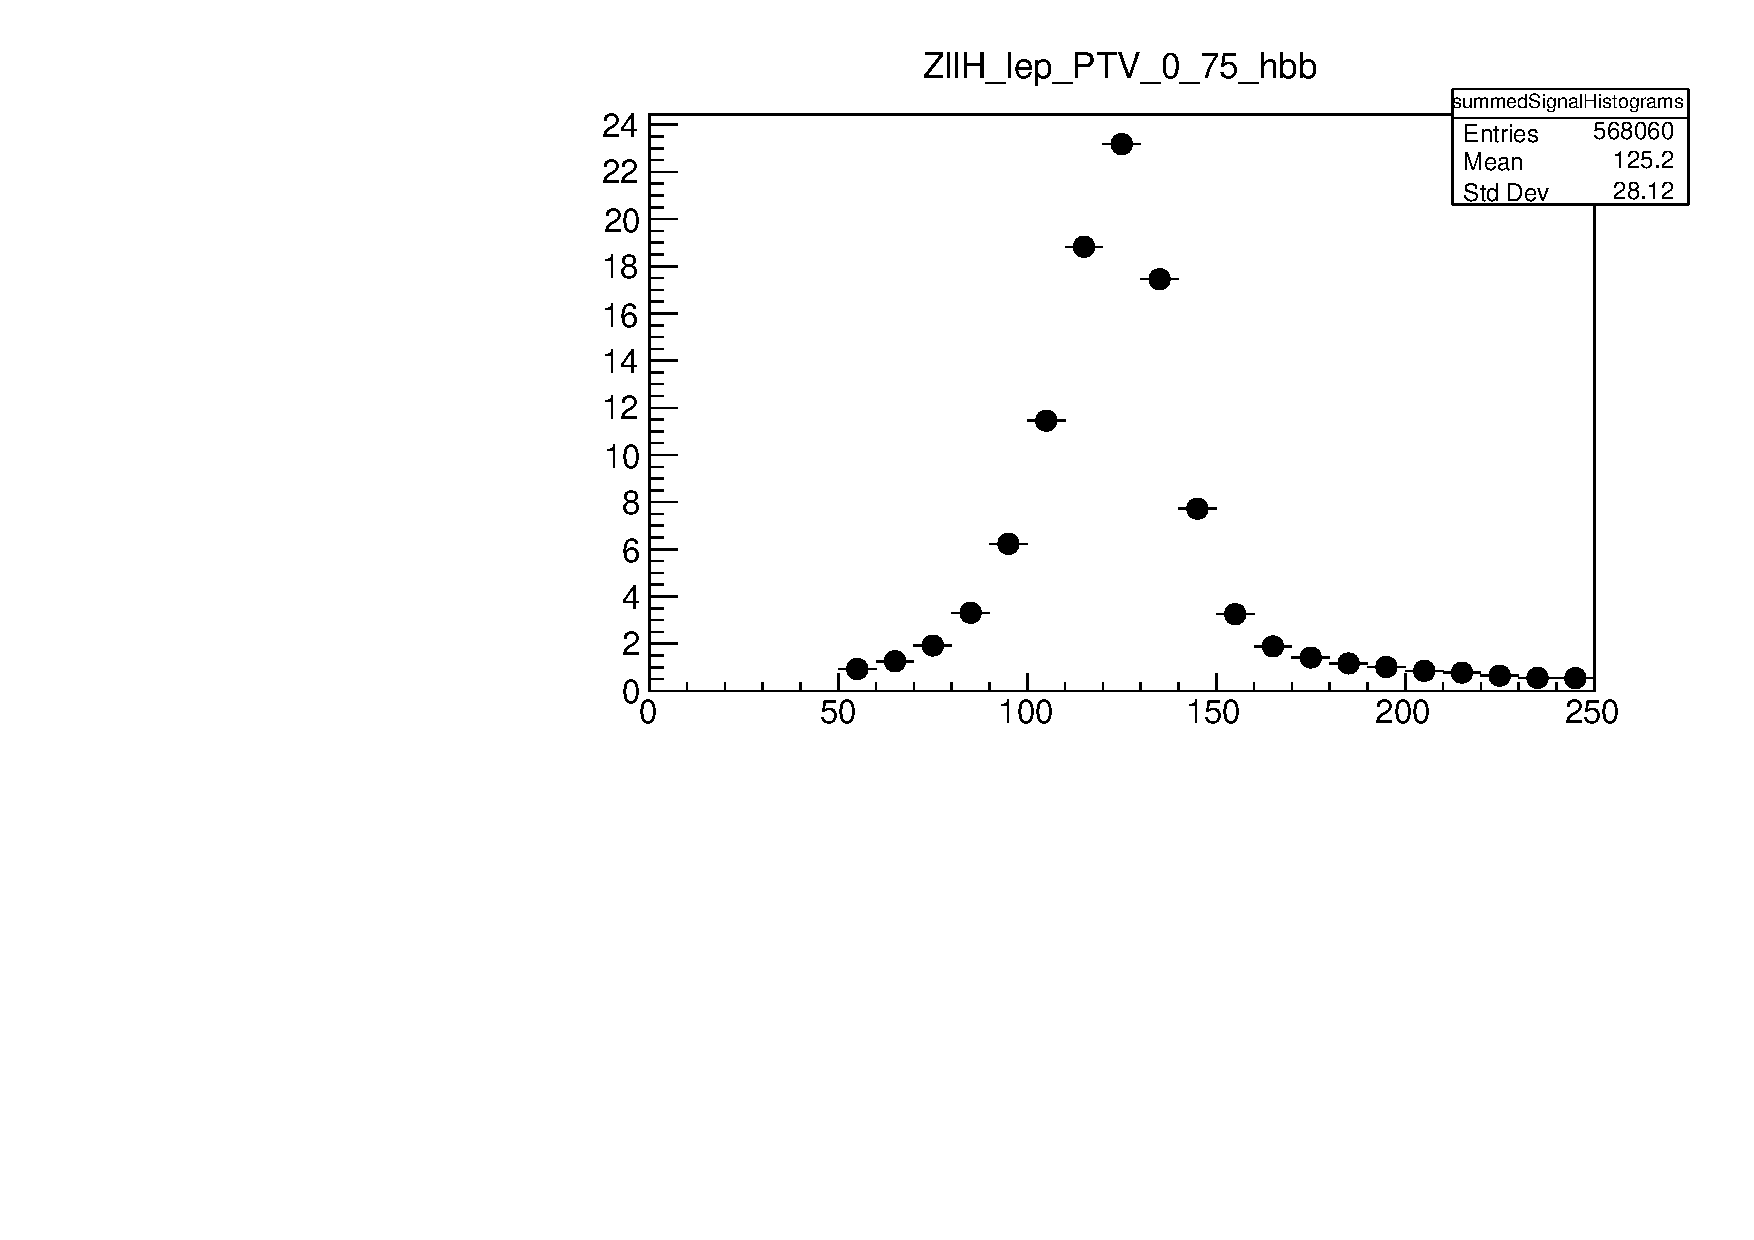
\includegraphics[width=\linewidth]{figs/reg.pdf}
    \end{column}
    \begin{column}{0.33\linewidth}
      \centering
      \textcolor{blue}{With Kinematic Fit}
      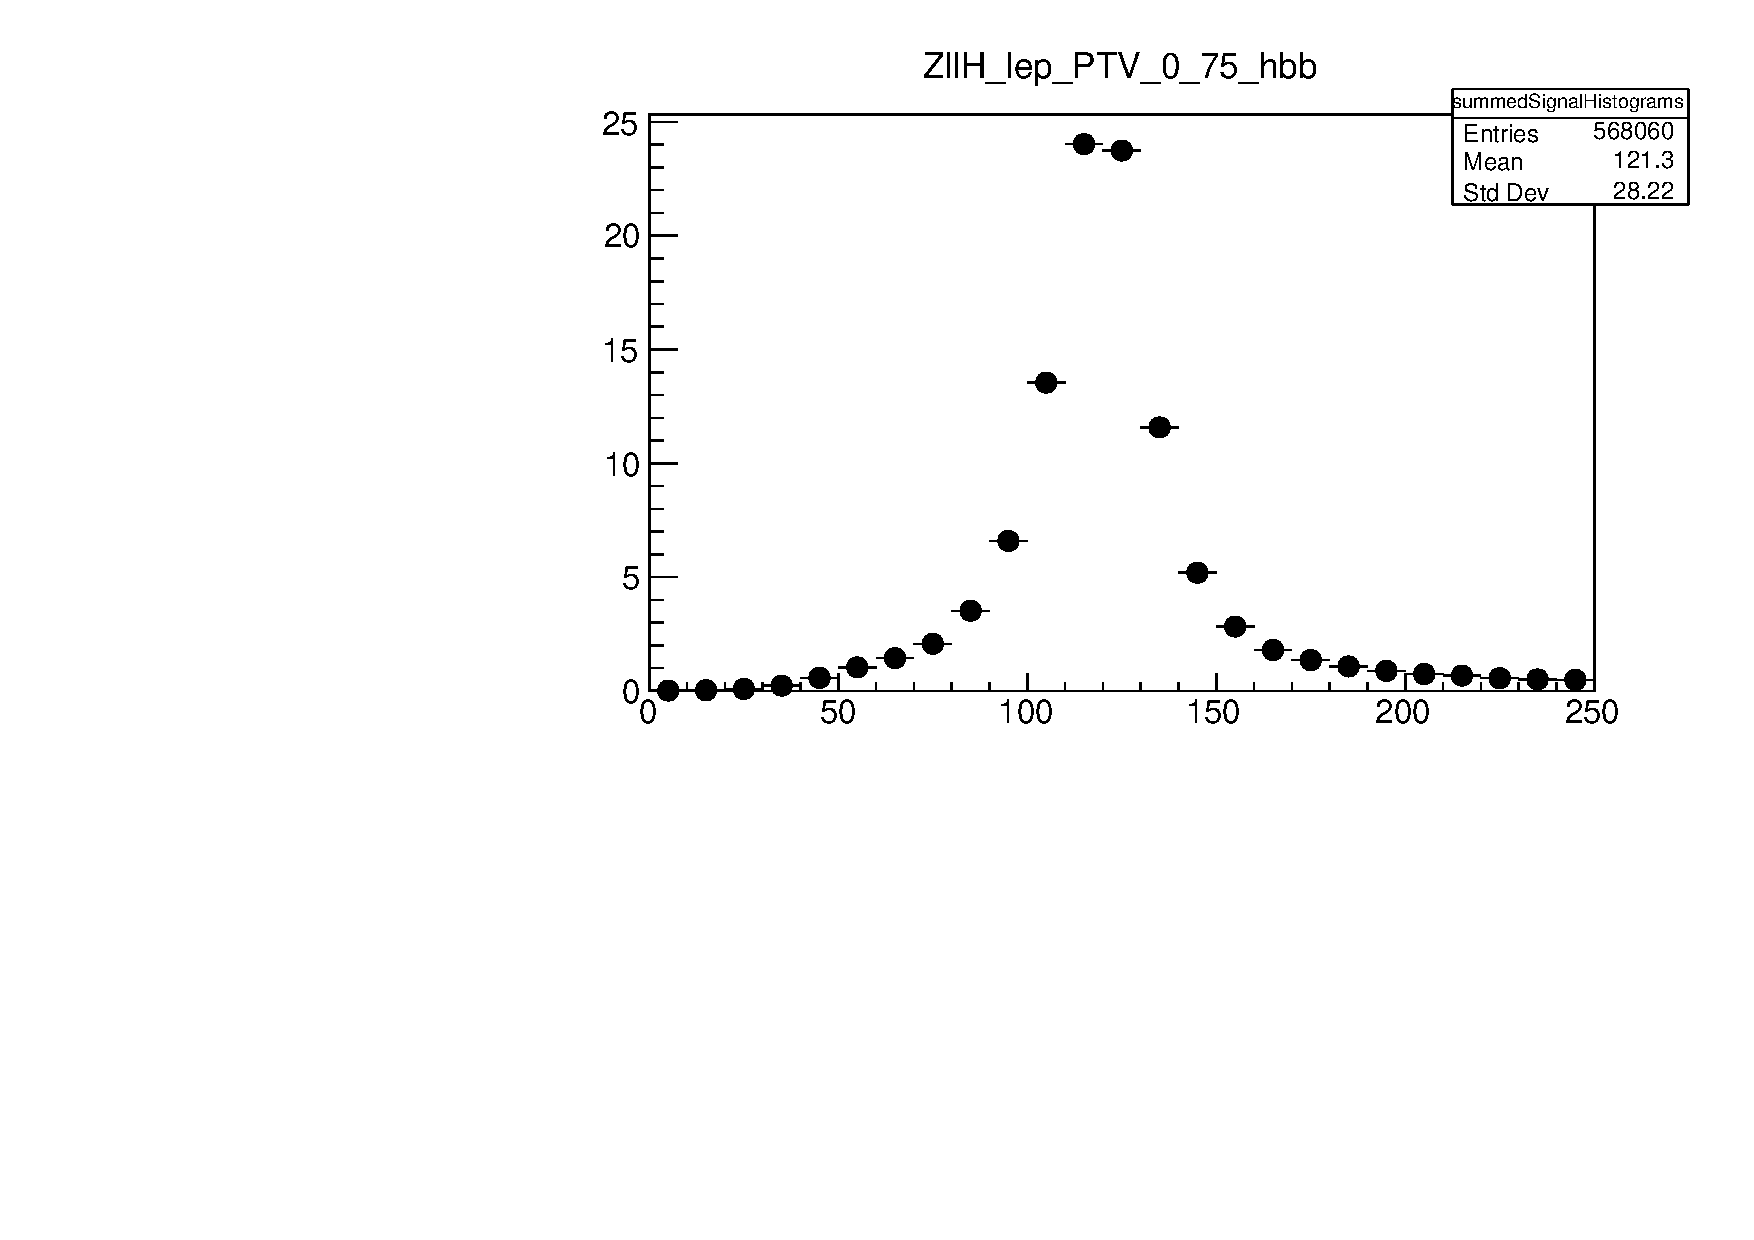
\includegraphics[width=\linewidth]{figs/kinfit.pdf}
    \end{column}
  \end{columns}

\end{frame}

\begin{comment}
\beginbackup

\begin{frame}
  \centering
    {\Huge \bf\sffamily Backup Slides}
\end{frame}

\begin{frame}
   \frametitle{\small 190611/plot\_time\_60000\_wide}
   \centering
   \includegraphics[width=0.6\linewidth]{190611/plot_time_60000_wide.pdf}
\end{frame}

\begin{frame}
   \frametitle{\small 190611/plot\_time\_wide}
   \centering
   \includegraphics[width=0.6\linewidth]{190611/plot_time_wide.pdf}
\end{frame}

\begin{frame}
   \frametitle{\small 190611/plot\_time\_120000\_compare}
   \centering
   \includegraphics[width=0.6\linewidth]{190611/plot_time_120000_compare.pdf}
\end{frame}

\begin{frame}
   \frametitle{\small 190611/plot\_time\_60000\_compare}
   \centering
   \includegraphics[width=0.6\linewidth]{190611/plot_time_60000_compare.pdf}
\end{frame}

\begin{frame}
   \frametitle{\small 190611/plot\_time\_80000\_compare}
   \centering
   \includegraphics[width=0.6\linewidth]{190611/plot_time_80000_compare.pdf}
\end{frame}

\begin{frame}
   \frametitle{\small 190611/plot\_time\_120000\_narrow}
   \centering
   \includegraphics[width=0.6\linewidth]{190611/plot_time_120000_narrow.pdf}
\end{frame}

\begin{frame}
   \frametitle{\small 190611/plot\_time\_40000\_narrow}
   \centering
   \includegraphics[width=0.6\linewidth]{190611/plot_time_40000_narrow.pdf}
\end{frame}

\begin{frame}
   \frametitle{\small 190611/plot\_time\_160000\_narrow}
   \centering
   \includegraphics[width=0.6\linewidth]{190611/plot_time_160000_narrow.pdf}
\end{frame}

\begin{frame}
   \frametitle{\small 190611/plot\_time\_60000\_narrow}
   \centering
   \includegraphics[width=0.6\linewidth]{190611/plot_time_60000_narrow.pdf}
\end{frame}

\begin{frame}
   \frametitle{\small 190611/plot\_time\_80000\_narrow}
   \centering
   \includegraphics[width=0.6\linewidth]{190611/plot_time_80000_narrow.pdf}
\end{frame}

\begin{frame}
   \frametitle{\small 190611/plot\_time\_narrow}
   \centering
   \includegraphics[width=0.6\linewidth]{190611/plot_time_narrow.pdf}
\end{frame}



\backupend
\end{comment}

\end{document}
